\chapter{Introduzione alle reti neurali}

Le reti neurali, grazie alla loro capacità di gestire dati non lineari e molto rumorosi, e di riconoscere pattern complessi, ritrovano moltissime applicazioni per la risoluzione di task di vario tipo. Esistono inoltre numerose varianti delle reti neurali (profonde e non), tra cui la MLP (di cui parleremo) e la CNN.


\section{Definizione di rete neurale}
Una rete neurale è una funzione matematica \textit{annidata} del tipo:

$$
f_n(f_{n-1}(\dots (f_1(x))))
$$

dove $n$ coincide col numero di strati, o \textit{layer}. Questa rete neurale ritorna uno scalare $y$.  Una rete neurale è quindi ottenuta da una \textbf{composizione di funzioni derivabili}. Le funzioni sono dette \textbf{funzioni di attivazione}, e andremo a vederne presto alcuni esempi.

\begin{figure}[tbph]
	\centering
	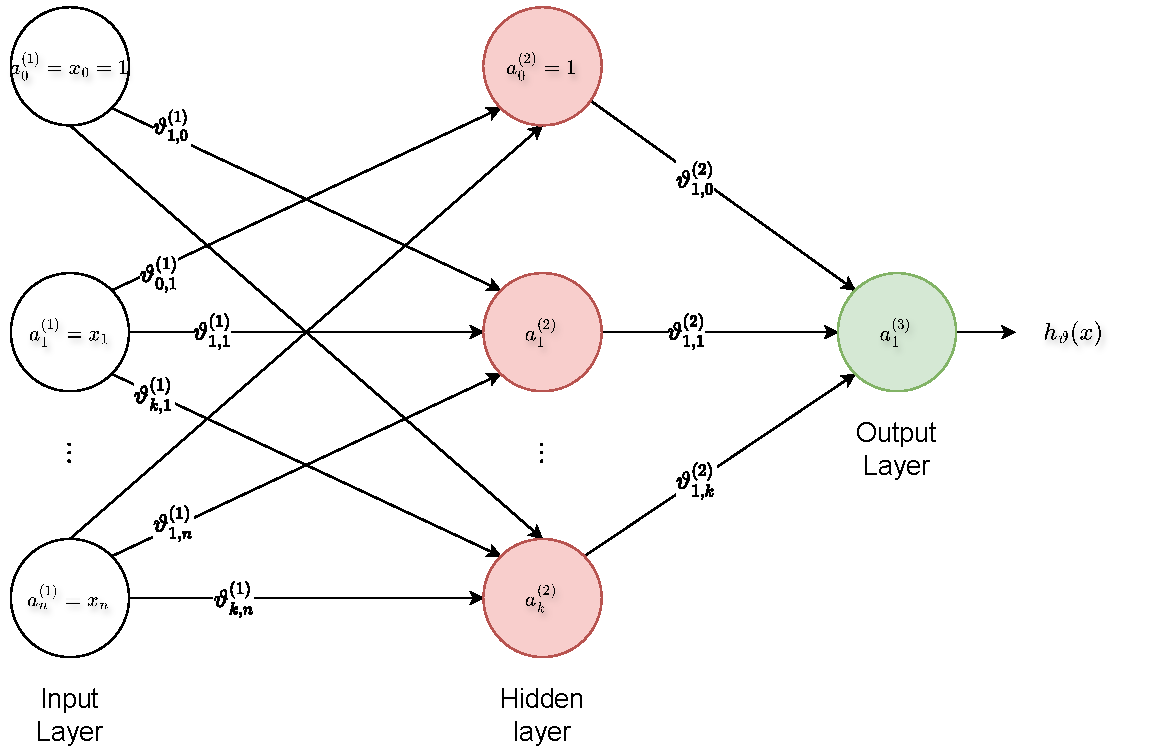
\includegraphics[width=0.8\linewidth]{images/NeuralNet1pdf}
	\caption{Un multilayer perceptron, ossia una particolare rete neurale.}
\end{figure}

Gli strati si suddividono in:

\begin{itemize}
	\item \textbf{Input Layer:} $a_0^{(1)}, a_1^{(1)}, \dots, a_n^{(1)}$. Ciascuno degli input viene moltiplicato per il rispettivo peso della coppia input-hidden layer. Questo viene realizzato tramite un prodotto righe per colonne tra la matrice dei pesi di ciascuno degli elementi dell'hidden layer, con i parametri d'input.
	
	\item \textbf{Hidden Layer:} sono tutti i layer che non sono né input né output. Il numero di hidden layer definisce la profondità della rete neurale. Una rete neurale si dice profonda (deep) quando si hanno $2 \leq$ hidden layers. Il numero di neuroni può cambiare da layer a layer. Il layer $n$-esimo comunica col layer $n+1$-esimo.
	
	\item \textbf{Output Layer:} riunisce i dati in output. La funzione di attivazione dell'output layer dipende fortemente dal tipo di task. Tra queste funzioni, abbiamo ad esempio la sigmoide, la tangente iperbolica, la softplus o la ReLU. 

\end{itemize}

Nelle reti neurali, individuiamo due parti fondamentali:

\begin{figure}[tbph]
	\centering
	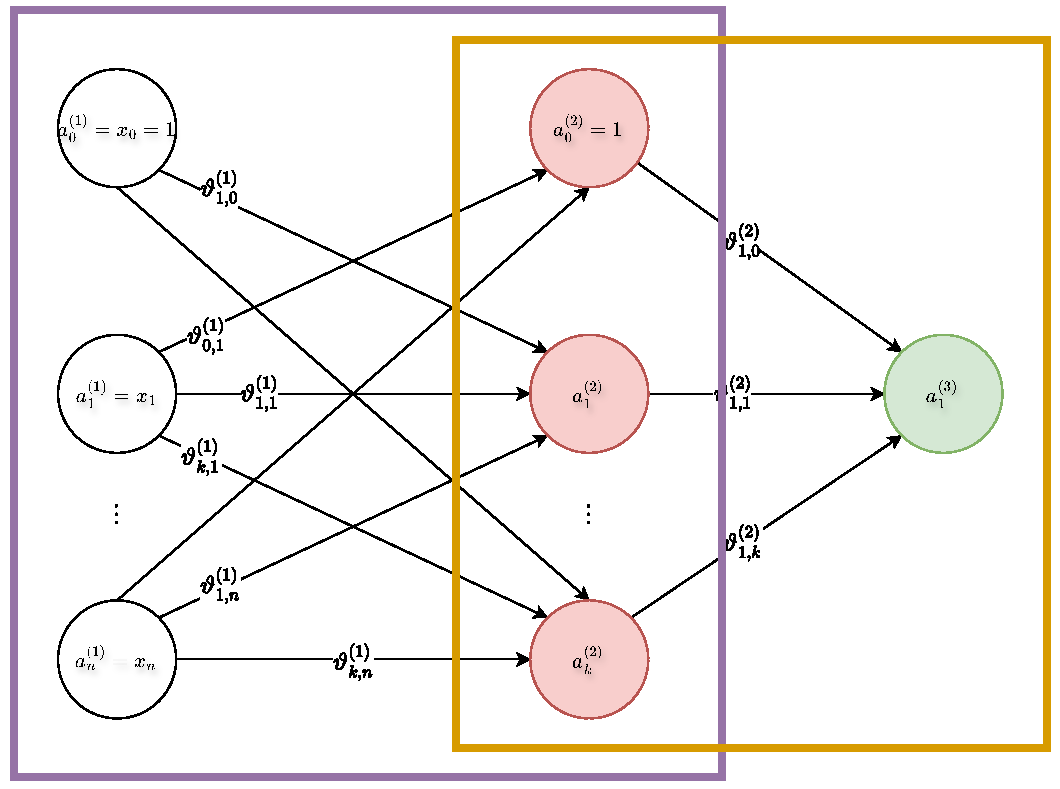
\includegraphics[width=0.75\linewidth]{images/NeuralNet2pdf}
	\caption{Un multilayer perceptron}
\end{figure}

Nella rete neurale fornita, individuiamo due parti.

\begin{itemize}
	\item La parte in viola della rete è dedicata alla \textbf{trasformazione degli input grezzi} in qualcosa di utile per il task. La trasformazione viene appresa in fase di training grazie alle etichette note dell'apprendimento supervisionato. In questo caso, permette di trasformare $x \to a^{(2)}$.
	
	\item La parte arancione invece è dedicata alla \textbf{classificazione} (tramite softmax, o regressore logistico nella classificazione binaria), prendendo come input i dati trasformati dal resto della rete, in questo caso $a^{(2)}$. Basta sostituire il softmax con un regressore lineare per usare la rete su task di regressione.
\end{itemize}


\section{Le funzioni di attivazione}
Le funzioni di attivazione devono essere derivabili per consentire il training della rete tramite algoritmo di backpropagation. Tra le funzioni più usate, abbiamo:

\begin{table}[ht]
	\centering
	\resizebox{\textwidth}{!}{%
		\begin{tabular}{lll}
			\hline
			\textbf{Nome} & \textbf{Equazione} & \textbf{Derivata} \\
			\hline
			Identità &
			$ f(x) = x $ &
			$ f'(x) = 1 $ \\[4pt]
			
			Gradino binario (Binary step) &
			$ f(x) =
			\begin{cases}
				0 & \text{per } x < 0,\\
				1 & \text{per } x \ge 0
			\end{cases} $ &
			$ f'(x) =
			\begin{cases}
				0 & \text{per } x \neq 0,\\
				? & \text{per } x = 0
			\end{cases} $ \\[8pt]
			
			Logistica (o Soft step) &
			$ f(x) = \dfrac{1}{1 + e^{-x}} $ &
			$ f'(x) = f(x)\bigl(1 - f(x)\bigr) $ \\[8pt]
			
			TanH &
			$ f(x) = \tanh(x) = \dfrac{2}{1 + e^{-2x}} - 1 $ &
			$ f'(x) = 1 - f(x)^2 $ \\[8pt]
			
			ArcTan &
			$ f(x) = \tan^{-1}(x) $ &
			$ f'(x) = \dfrac{1}{x^2 + 1} $ \\[8pt]
			
			Unità lineare rettificata (ReLU) &
			$ f(x) =
			\begin{cases}
				0 & \text{per } x < 0,\\
				x & \text{per } x \ge 0
			\end{cases} $ &
			$ f'(x) =
			\begin{cases}
				0 & \text{per } x < 0,\\
				1 & \text{per } x \ge 0
			\end{cases} $ \\[8pt]
			
			Unità lineare rettificata parametrica (PReLU) &
			$ f(x) =
			\begin{cases}
				\alpha x & \text{per } x < 0,\\
				x        & \text{per } x \ge 0
			\end{cases} $ &
			$ f'(x) =
			\begin{cases}
				\alpha & \text{per } x < 0,\\
				1      & \text{per } x \ge 0
			\end{cases} $ \\[8pt]
			
			Unità lineare esponenziale (ELU) &
			$ f(x) =
			\begin{cases}
				\alpha\left(e^{x} - 1\right) & \text{per } x < 0,\\
				x                            & \text{per } x \ge 0
			\end{cases} $ &
			$ f'(x) =
			\begin{cases}
				f(x) + \alpha & \text{per } x < 0,\\
				1             & \text{per } x \ge 0
			\end{cases} $ \\[8pt]
			
			SoftPlus &
			$ f(x) = \log_e\!\bigl(1 + e^{x}\bigr) $ &
			$ f'(x) = \dfrac{1}{1 + e^{-x}} $ \\[4pt]
			\hline
		\end{tabular}%
	}
\end{table}

Riportiamo alcuni dei plotting delle funzioni di attivazione e le loro derivate. 

\begin{figure}[tbph]
	\centering
	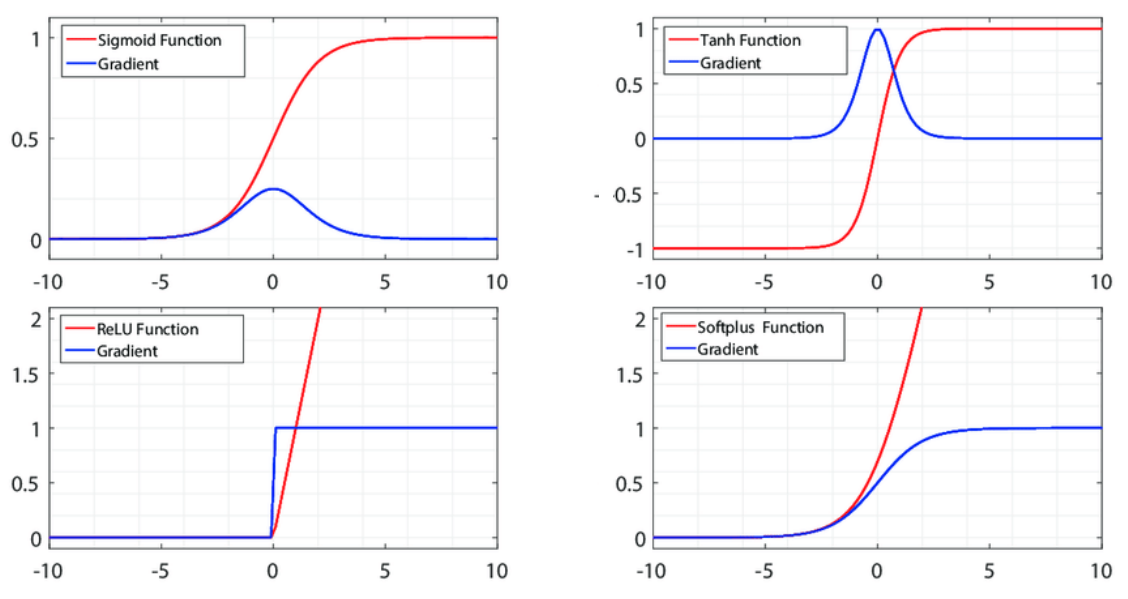
\includegraphics[width=1\linewidth]{images/activation-functions}
\end{figure}

\subsection{Il teorema di approssimazione universale - \textit{Universal Approximation Theorem}}
Il teorema di approssimazione universale afferma che una rete neurale con un singolo strato nascosto può approssimare qualsiasi funzione continua con un livello di precisione arbitrario. Il layer potrebbe tuttavia essere estremamente numeroso e potrebbe soffrire di overfitting.


\section{Training e inferenza di una rete neurale}
\begin{figure}[tbph]
	\centering
	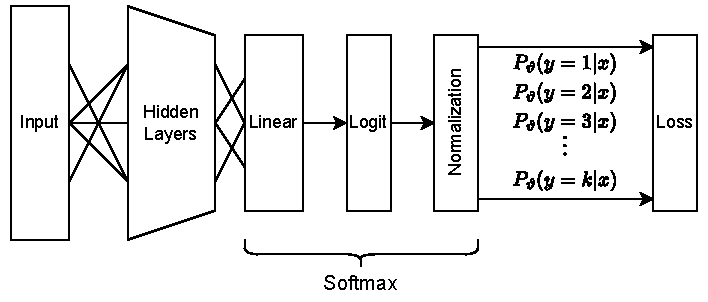
\includegraphics[width=1\linewidth]{images/neural-net}
	\caption{Struttura tipica di una rete neurale per la classificazione.}
\end{figure}

Durante la fase di training, il nostro obiettivo è quello di stabilire i migliori parametri per il nostro modello sui dati di training. Usiamo quindi la Loss function e la nostra procedura di training. Usiamo poi il modello con i parametri ottenuti per fare inferenza su nuovi dati, e osservare le performance del modello.


\subsection{Funzione di costo}
Definiamo la nostra funzione di costo.

$$
J(\vartheta) = -\frac{1}{m} \sum_{i=1}^{m} \underbrace{\sum_{c=1}^{k}\mathbf{1}\{y^{(i)} = c\} \log(h_\vartheta^{(c)}(x^{(i)}))}_\text{Cross Entropy Loss Function}
$$

\noindent 
in cui
\begin{itemize}
	\item $m$ = numero di esempi nel dataset
	\item $k$ = numero di classi
	\item $(x^{(i)})$ = $i$-esimo input
	\item $(y^{(i)})$ = etichetta (classe corretta) dell’$i$-esimo esempio
	\item $(\mathbf{1}(y^{(i)} = c))$ = funzione indicatrice: vale 1 se l’esempio ($i$) appartiene alla classe ($c$), altrimenti 0
	\item $(h_\theta^{(c)}(x^{(i)}))$ = output della rete (probabilità predetta) per la classe ($c$) sull’esempio ($i$)
\end{itemize}

\noindent
Il nostro obiettivo è quello di trovare $\hat{\vartheta}$, ossia i valori dei parametri $\vartheta$, tali che
$$
\hat\vartheta = \min(J(\vartheta))
$$


\subsection{Chain Rule}
Considerando le reti neurali come delle funzioni composte, o annidate, è possibile usare la chain rule per le derivate di funzioni composte.

$$
\frac{\partial J(\vartheta)}{\partial\vartheta_{i,j}^{(l)}} \quad \forall j, i, l
$$ 


\subsection{Inizializzazione dei parametri}
L'inizializzazione dei parametri avviene con numeri casuali molto piccoli $\in [-\varepsilon, +\varepsilon]$. I parametri dei nodi che dipendono dallo stesso nodo, devono essere diversi tra loro, effettuando quella che è nota come \textbf{simmetry breaking}. Valori uguali sui nodi, porteranno i nodi a comportarsi in maniera simile, rendendo inutile avere modelli più complessi.


\subsection{Reti neurali per regressione}
Usiamo come Loss function l'errore quadratico medio (MSE). Ogni output sarà un regressore lineare, e la Loss function valuterà gli output di tutti i regressori.
\begin{figure}[tbph]
	\centering
	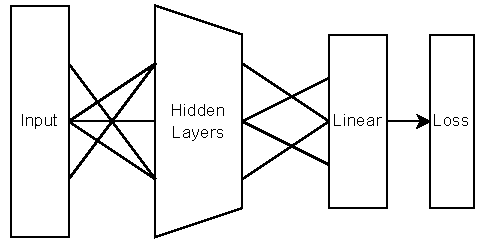
\includegraphics[width=0.8\linewidth]{images/linear-reg-neuralnet}
\end{figure}


\section{Overfitting e Underfitting nelle reti neurali}
\paragraph{Underfitting.} Le reti neurali più piccole, su dati molto complessi, sono soggette ad underfitting. I pochi parametri non permettono di descrivere (o separare) i pattern complessi dei dati. Si riscontrano alti errori già in fase di training. Reti più semplici sono però più veloci da allenare.

\paragraph{Overfitting.} Le reti neurali più complesse, con tanti parametri, imparano meglio i dati in fase di training, minimizzando o addirittura azzerando la loss function. Il rischio è opposto: il modello diventa troppo specifico, e non riesce a generalizzare sui dati di testing, cascando in overfitting. Diventa quindi necessario introdurre termini di regolarizzazione ($\lambda$) o cambiare modello. Modelli più vasti richiedono inoltre risorse computazionali più importanti.


